% Created 2023-05-15 lun 23:28
% Intended LaTeX compiler: pdflatex
\documentclass[letterpaper, 11pt]{article}
                      \usepackage{lmodern} % Ensures we have the right font
\usepackage[T1]{fontenc}
\usepackage[utf8]{inputenc}
\usepackage{sectsty}
\usepackage{graphicx}
\usepackage{amsmath, amsthm, amssymb}
\usepackage[table, xcdraw]{xcolor}
\pagestyle{fancy}
\usepackage{multicol}
\setlength\columnsep{25pt} % This is the default columnsep for all pages
\definecolor{bblue}{HTML}{0645AD}
\usepackage[colorlinks]{hyperref}
\usepackage[dvipsnames]{xcolor}
\hypersetup{colorlinks, linkcolor=blue, urlcolor=bblue}
\usepackage{titling}
\setlength{\droptitle}{-6em}
\setlength{\parindent}{0pt}
\setlength{\parskip}{1em}
\usepackage[stretch=10]{microtype}
\usepackage{hyphenat}
\usepackage{ragged2e}
\usepackage{subfig} % Subfigures (not needed in Org I think)
\usepackage{hyperref} % Links
\usepackage{listings} % Code highlighting
\usepackage[top=0.6in, bottom=1.25in, left=0.4in, right=0.4in]{geometry}
\renewcommand{\baselinestretch}{1.15}
\usepackage[explicit]{titlesec}
\pretitle{\begin{center}\fontsize{20pt}{20pt}\selectfont}
\posttitle{\par\end{center}}
\preauthor{\begin{center}\vspace{-6bp}\fontsize{14pt}{14pt}\selectfont}
\postauthor{\par\end{center}\vspace{-25bp}}
\predate{\begin{center}\fontsize{12pt}{12pt}\selectfont}
\postdate{\par\end{center}\vspace{-3em}}
\titlespacing\section{0pt}{5pt}{5pt} % left margin, space before section header, space after section header
\titlespacing\subsection{0pt}{5pt}{-2pt} % left margin, space before subsection header, space after subsection header
\titlespacing\subsubsection{0pt}{5pt}{-2pt} % left margin, space before subsection header, space after subsection header
\usepackage{enumitem}
\setlist{itemsep=-2pt} % or \setlist{noitemsep} to leave space around whole list
\author{Matteo Lugli, Carlo Uguzzoni}
\date{\today}
\title{LoopFusion}
\hypersetup{
 pdfauthor={Matteo Lugli, Carlo Uguzzoni},
 pdftitle={LoopFusion},
 pdfkeywords={},
 pdfsubject={},
 pdfcreator={Emacs 27.1 (Org mode 9.3)}, 
 pdflang={English}}
\begin{document}

\maketitle
\tableofcontents

\newpage
\begin{multicols}{2}
\section{Requisiti per la loop fusion}
\label{sec:org7ed5afc}
Si supponga che si stiano prendendo in considerazione i due loop CFG equivalenti
\(L_{i}\) e \(L_{k}\).
\subsection{Adiacenza}
\label{sec:org64c18cc}
L'adiacenza dei due loop viene verificata controllando \emph{(i)} che l'\textbf{exit block} di
\(L_{i}\) corrisponda all'\textbf{header} di \(L_{k}\) \emph{(ii)} e che il suddetto blocco di intersezione
contenga soltanto un'istruzione di tipo \textbf{branch}, la cui destinazione deve essere necessariamente
il \textbf{body} di \(L_{k}\).
Esiste anche il caso in cui i due loop non sono immediatamente adiacenti, ma lo
potrebbero diventare applicando adeguate operazioni di trasformazione. Questo
non viene gestito per semplicità, dato che richederebbe un'analisi piuttosto avanzata.
\footnotesize
\begin{verbatim}
if (L1->getExitBlock() == L2->getLoopPreheader()) {
  int instruction_count = 0;
  BasicBlock *MiddleBlock = L1->getExitBlock();

  for (auto iter_block = MiddleBlock->begin(); 
	   iter_block != MiddleBlock->end(); 
	   ++iter_block) {
	   ++instruction_count;
  }
  if (instruction_count != 1) {
	continue;
  }
  Instruction *I = dyn_cast<Instruction> 
	  (MiddleBlock->begin());
  BranchInst *BI = dyn_cast<llvm::BranchInst> (I);
  if (!(BI && BI->getSuccessor(0)== L2->getHeader())) {
	continue;
  }
\end{verbatim}
\normalsize
\subsection{Trip count}
\label{sec:org1427caf}
Serve inoltre verificare che \(L_{i}\) e \(L_{k}\) eseguano in ogni caso
lo stesso numero di iterazioni, quindi che abbiano lo stesso trip count.
Per esegure questo controllo è necessaria un'analisi preliminare, che
in LLVM prende il nome di \textbf{ScalarEvolutionAnalysis}. Si può ottenere
chiamando l'apposito metodo del \textbf{FunctionAnalysisManager}: 
\footnotesize
\begin{verbatim}
auto &SE = AM.getResult<ScalarEvolutionAnalysis>(F);
\end{verbatim}
\normalsize
\subsection{Dipendenze}
\label{sec:org22ad388}
\section{Esecuzione della loop fusion}
\label{sec:org24525b4}
Se \(L_{i}\) e \(L_{k}\) hanno superato tutti i controlli, si può
procedere ad effettuare la loop fusion.
In LLVM il modo più semplice per modificare il \emph{control flow} del programma
è cambiare la direzione degli archi del grafo. Le operazioni da eseguire sono
le seguenti: \emph{(i)} collegare l'ultimo BB\footnote{Basic Block} del \emph{body} di \(L_{i}\) al
primo BB del \emph{body} di \(L_{k}\),
\footnotesize
\begin{verbatim}
// save this final block for later
BasicBlock *FINAL = L2->getExitBlock();

BasicBlock *LL1 = L1->getLoopLatch();
BasicBlock *LB1 = LL1->getPrevNode();
BasicBlock *HB2 = L2->getHeader();
Instruction* L2PHI = dyn_cast<Instruction>(HB2->begin());
Instruction *I1 = HB2->getTerminator();        
BranchInst *BI1 = dyn_cast<llvm::BranchInst>(I1);
BasicBlock *LB2 = BI1->getSuccessor(0);
Instruction *I2 = LB1->getTerminator();
BranchInst *BI2 = dyn_cast<llvm::BranchInst>(I2);
BI2->setSuccessor(0, LB2);
\end{verbatim}
\normalsize
 \emph{(ii)} il \emph{body} di \(L_{k}\) al \emph{latch} di \(L_{i}\),
\footnotesize
\begin{verbatim}
BasicBlock *LL2 = L2->getLoopLatch();
BasicBlock *LB2E = LL2->getPrevNode();
Instruction *LB2E_branch = LB2E->getTerminator();
LB2E_branch->setSuccessor(0,LL1);
\end{verbatim}
\normalsize
\emph{(iii)} il ramo \emph{false} dell'\emph{header} di \(L_{i}\) con l'\emph{exit block} di \(L_{k}\).
\footnotesize
\begin{verbatim}
BasicBlock *HB1 = L1->getHeader();
Instruction *I4 = HB1->getTerminator();
BranchInst *BI4 = dyn_cast<llvm::BranchInst>(I4);
BI4->setSuccessor(1, FINAL);
\end{verbatim}
\normalsize
Le trasformazioni sono ben visibili in Figura 1 e in Figura 2.
Infine si sostituiscono tutti gli usi della \emph{induction variable} di \(L_{k}\) con 
l'\emph{induction variable} di \(L_{i}\), in modo da usarne soltanto una per gestire le operazioni
di entrambi i loop, che ora possono essere considerati uno solo.
\newpage
\footnotesize
\begin{verbatim}
Instruction* L1PHI = dyn_cast<Instruction>(HB1->begin());
Value *CastedL1PHI = dyn_cast<Value>(L1PHI);
L2PHI->replaceAllUsesWith(CastedL1PHI);
L2PHI->eraseFromParent();
\end{verbatim}
\normalsize
A seguito della qui discussa ottimizzazione, alcuni BB rimangono scollegati dal resto del
CFG, risultando quindi inacessibili. In Figura 2 compaiono nella categoria "Garbage Blocks".
Da notare in particolare il \emph{latch} di \(L_{k}\), che se lasciato avrebbe comportato il
doppio incremento della \emph{induction variable}.
\newpage
\end{multicols}
\begin{figure}[htbp]
\centering
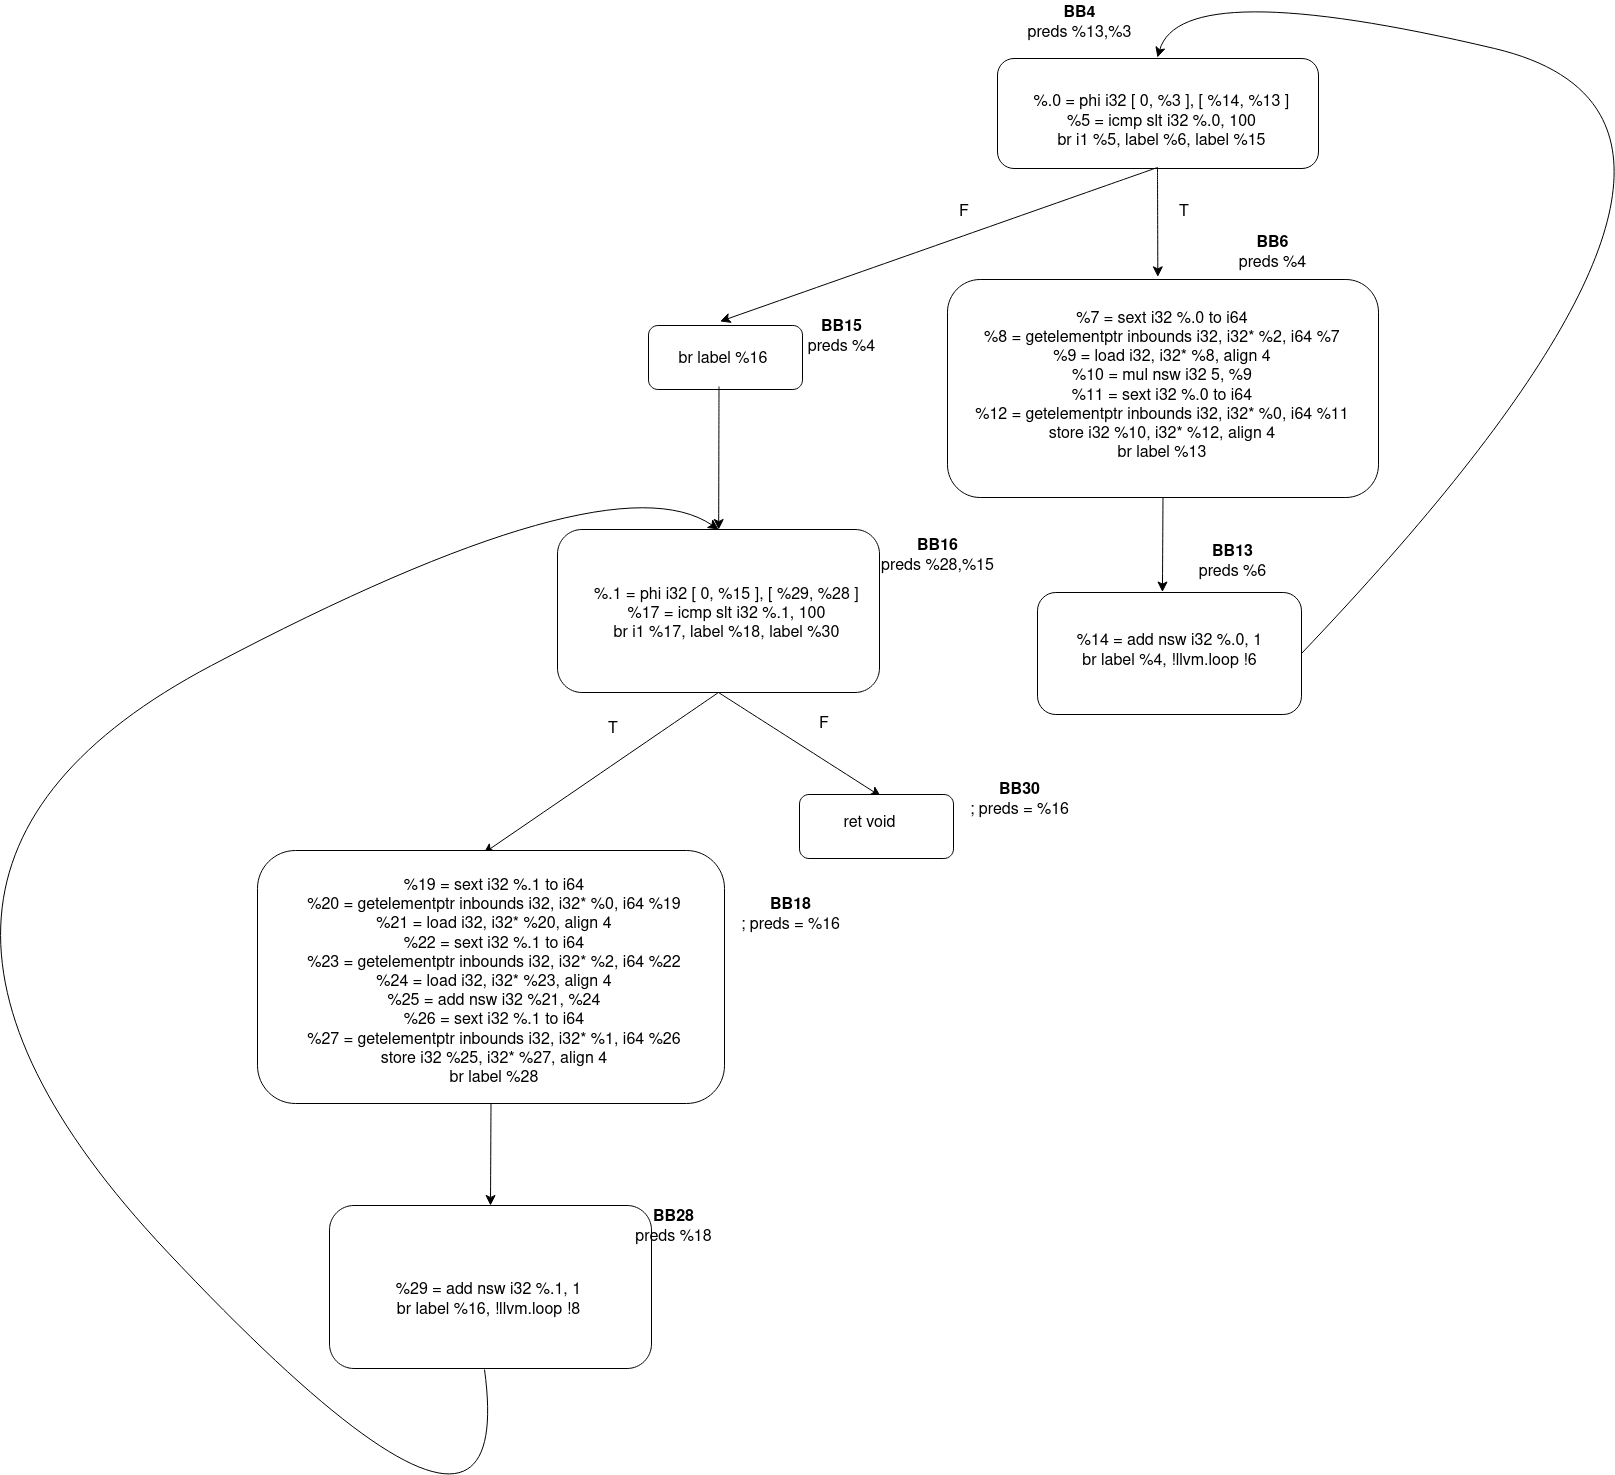
\includegraphics[width=20cm]{/home/eros/Downloads/bfore.png}
\caption{CFG prima del passo di ottimizzazione}
\end{figure}
\begin{figure}[htbp]
\centering
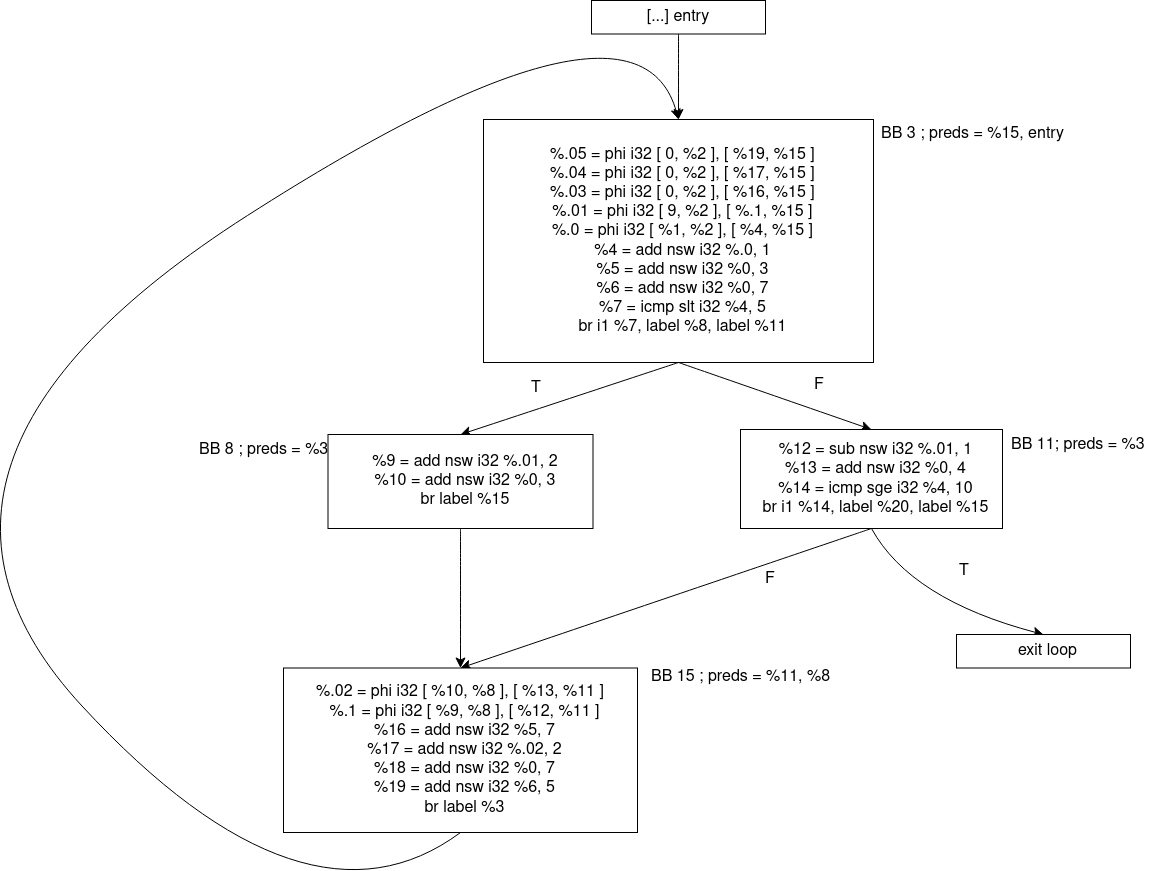
\includegraphics[width=20cm]{/home/eros/Downloads/after.png}
\caption{CFG dopo il passo di ottimizzazione}
\end{figure}
\end{document}
